
\begin{frame}{1.4绝对值}
\mbox{我们把在数轴上表示数$a$的点与原点的距离叫做数$a$的绝对值, 记作|$a$|.}
\begin{columns}
\column{0.45\textwidth}
\begin{enumerate}[label={\arabic*.}]
\item 一个正数的绝对值是它本身; 
\item 0 的绝对值是0;
\item 一个负数的绝对值是它的相反数.
\end{enumerate}

\begin{itemize}
    \item \textbf{数学表达式}:  $\left|  x  \right|$
    \item  \textbf{函数定义}: \[ f(x) = \begin{cases}
    x, x>0 \\
    0, x=0 \\
    -x, x<0
    \end{cases}
    \]
    \item \textbf{定义域}: $x \in \mathbb{R}$
    \item \textbf{值域}: $y \in \mathbb{R}, y \geq 0$
    \item \textbf{对称性}: 关于y轴对称
\end{itemize}

%绝对值函数图象
\column{0.5\textwidth}
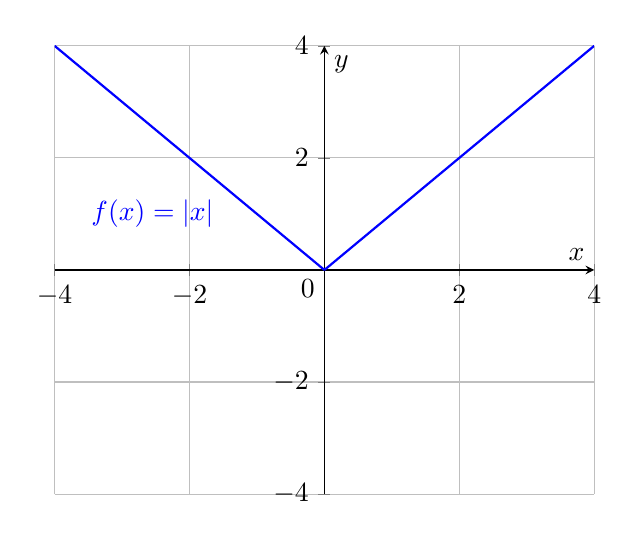
\begin{tikzpicture}[scale=1]
\begin{axis}[
    axis lines=middle,
    xlabel=$x$, ylabel=$y$,
    xmin=-4, xmax=4, ymin=-4, ymax=4,
    samples=500,
    grid=both,
    restrict y to domain=-10:10,
]
\addplot[blue, thick] {abs(x)};
\node[black] at (0,0) [below left] {0};
\node[blue] at (-1.5,1) [left] {$f(x)=|x|$};
\end{axis}
\end{tikzpicture}

\end{columns}
\end{frame}

% 绝对值与相反数的比较
\begin{frame}{绝对值与相反数的比较}
\begin{columns}

%相反数函数图象
\column{0.5\textwidth}
\textbf{相反数的函数图象}
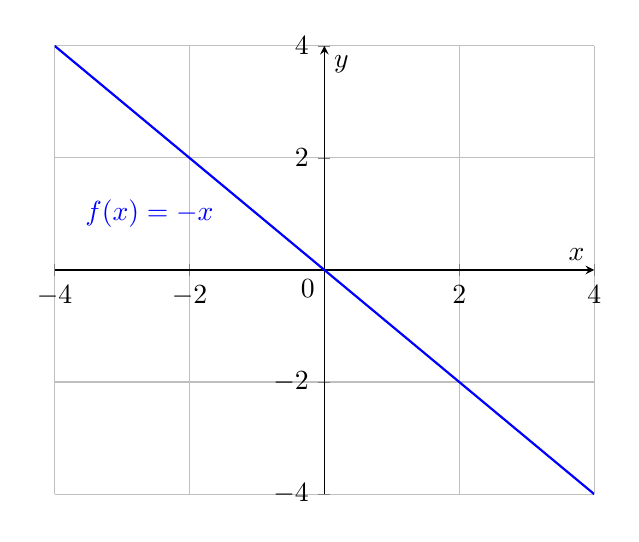
\begin{tikzpicture}[scale=1]
\begin{axis}[
    axis lines=middle,
    xlabel=$x$, ylabel=$y$,
    xmin=-4, xmax=4, ymin=-4, ymax=4,
    samples=500,
    grid=both,
    restrict y to domain=-10:10,
]
\addplot[blue, thick] {-x};
\node[black] at (0,0) [below left] {0};
\node[blue] at (-1.5,1) [left] {$f(x)=-x$};
\end{axis}
\end{tikzpicture}

%绝对值函数图象
\column{0.5\textwidth}
\textbf{绝对值的函数图象}
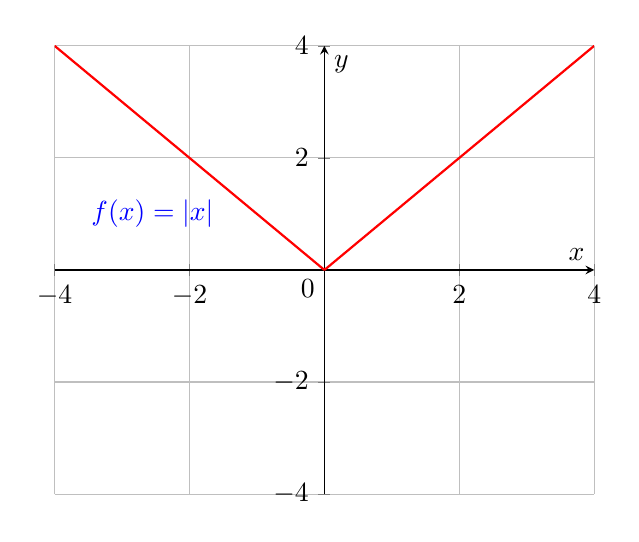
\begin{tikzpicture}[scale=1]
\begin{axis}[
    axis lines=middle,
    xlabel=$x$, ylabel=$y$,
    xmin=-4, xmax=4, ymin=-4, ymax=4,
    samples=500,
    grid=both,
    restrict y to domain=-10:10,
]
\addplot[red, thick] {abs(x)};
\node[black] at (0,0) [below left] {0};
\node[blue] at (-1.5,1) [left] {$f(x)=|x|$};
\end{axis}
\end{tikzpicture}
\end{columns}
\end{frame}

